\documentclass[ignorenonframetext,]{beamer}
\setbeamertemplate{caption}[numbered]
\setbeamertemplate{caption label separator}{: }
\setbeamercolor{caption name}{fg=normal text.fg}
\beamertemplatenavigationsymbolsempty
\usepackage{lmodern}
\usepackage{amssymb,amsmath}
\usepackage{ifxetex,ifluatex}
\usepackage{fixltx2e} % provides \textsubscript
\ifnum 0\ifxetex 1\fi\ifluatex 1\fi=0 % if pdftex
\usepackage[T1]{fontenc}
\usepackage[utf8]{inputenc}
\else % if luatex or xelatex
\ifxetex
\usepackage{mathspec}
\else
\usepackage{fontspec}
\fi
\defaultfontfeatures{Ligatures=TeX,Scale=MatchLowercase}
\fi
% use upquote if available, for straight quotes in verbatim environments
\IfFileExists{upquote.sty}{\usepackage{upquote}}{}
% use microtype if available
\IfFileExists{microtype.sty}{%
\usepackage{microtype}
\UseMicrotypeSet[protrusion]{basicmath} % disable protrusion for tt fonts
}{}
\newif\ifbibliography

% Prevent slide breaks in the middle of a paragraph:
\widowpenalties 1 10000
\raggedbottom

\AtBeginPart{
\let\insertpartnumber\relax
\let\partname\relax
\frame{\partpage}
}
\AtBeginSection{
\ifbibliography
\else
\let\insertsectionnumber\relax
\let\sectionname\relax
\frame{\sectionpage}
\fi
}
\AtBeginSubsection{
\let\insertsubsectionnumber\relax
\let\subsectionname\relax
\frame{\subsectionpage}
}

\setlength{\parindent}{0pt}
\setlength{\parskip}{6pt plus 2pt minus 1pt}
\setlength{\emergencystretch}{3em}  % prevent overfull lines
\providecommand{\tightlist}{%
\setlength{\itemsep}{0pt}\setlength{\parskip}{0pt}}
\setcounter{secnumdepth}{0}

\title{Simulationsbasierte Posteriori-Inferenz}
\author{Volker Schmid}
\date{19./26. Juni 2017}

\begin{document}
\frame{\titlepage}

\begin{frame}
\tableofcontents[hideallsubsections]
\end{frame}

\section{Einführung}\label{einfuhrung}

\begin{frame}{Zielsetzung}

Für komplexere Modelle ist die Posteriori of nicht mehr analytisch
zugänglich. Insbesondere ist die Normalisierungskonstante, d.h., die
marginale Likelihood \[
p(x)=\int f(x|\theta)p(\theta)d\theta
\] schwer zu berechnen. Auswege:

\begin{itemize}
\tightlist
\item
  Numerische Integration
\item
  Approximation der Posteriori
\item
  Simulationsverfahren
\end{itemize}

\end{frame}

\begin{frame}{Simulationsbasierte Posteriori-Inferenz}

Idee: Erzeuge Ziehungen aus der Posteriori-Verteilung und approximiere
daraus Statistiken der Posteriori-Verteilung

\begin{itemize}
\tightlist
\item
  Posteriori-Erwartungswert durch den Mittelwert
\item
  Posteriori-Median über Median der Stichprobe
\item
  Quantile der Posteriori-Verteilung über Quantile der Stichprobe
\item
  HPD-Intervalle als kürzeste Intervalle, die \(100(1-\alpha)\%\) der
  Stichprobe enthalten
\end{itemize}

\end{frame}

\section{Monte-Carlo-Integration}\label{monte-carlo-integration}

\begin{frame}{Definition}

Sei \(f(x)>0\) eine beliebige stetige Funktion mit bekanntem
Wertebereich \([0,Y]\). \(\int_a^b f(x) dx\) kann wie dann folgt
approximiert werden.

\begin{itemize}
\item Ziehe $n$ gleichverteilte Zufallszahlen $x$ aus $[a,b]$ 
\item Ziehe unabhängig davon $n$ gleichverteilte Zufallszahlen $y$ aus $[0,Y]$
\item Berechne den Anteil $h$ der Punkte $(x_i,y_i)$, die unterhalb der Funktion $f$ liegen 
\item $\int_a^b f(x) dx \approx h(b-a)Y$ 
\end{itemize}

\end{frame}

\begin{frame}{Beispiel}

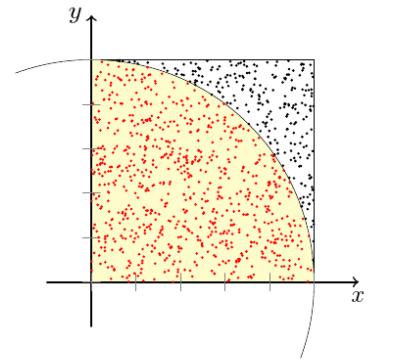
\includegraphics[scale=.4]{pics/mc-int.png}

\end{frame}

\begin{frame}[allowframebreaks]{Monte-Carlo-Schätzer}

Ist \(p(x)\) eine Dichte, so können Integrale der Form\[
E(g(x))=\int g(x)p(x) dx
\] mit einer Stichprobe \(x_1,\ldots,x_m\) aus \(p(x)\) durch den
Stichprobenmittelwert \[
\bar{g}_m=\frac{1}{m}\sum_{i=1}^mg\left(x_i\right)
\] approximiert werden. Aus dem starken Gesetz der grossen Zahlen folgt
\[
\lim \frac{1}{m} \sum_{i=1}^m g(x_i)\to \int g(x)p(x)dx.
\]

Die Varianz des Monte-Carlo-Schätzers \(\bar{g}_m\) ist gegeben durch \[
Var(\bar{g}_m)=\frac{1}{m}\int\left(g(X)-E(g(x))\right)^2 p(x)dx=\frac{1}{m}Var(g).
\] Der Approximationsfehler verringert sich mit steigendem \(m\). Es
folgt sogar aus dem zentralen Grenzwertsatz \[
\sqrt{m}\left(g_m-E(g(x))\right)\sim N(0,Var(g)).
\] Schätzer für \(Var(\bar{g}_m)\) ist
\[ \widehat{Var(\bar{g}_m)}=\frac{1}{m-1}\sum_{i=1}^m
\left(g(x_i)-\bar{g}_m\right)^2
\]

\end{frame}

\section{Ziehen von Zufallsvariablen}\label{ziehen-von-zufallsvariablen}

\begin{frame}{Inversionsmethode}

Gegeben sei die Verteilungsfunktion \(F(x)\) einer Zufallsvariablen
\(X\). Sei \(u\sim U[0,1]\). Dann ist \[
Y = F^{-1}(u) = \inf\{y:F(y)\geq u\} \sim X
\]

\end{frame}

\begin{frame}{Acception-Rejection-Methode}

Ziel: Wir wollen aus einer Dichtefunktion \(f(x)\) ziehen. Gegeben sei
eine Dichtefunktion \(g(x)\), nach der wir problemlos Zufallszahlen
ziehen können. Es existiere ein \(c\), so dass \[
cg(z)\geq f(z)
\] für alle \(z\) mit \(f(z)>0\). Dann können Zufallszahlen gemäß
\(f(x)\) wie folgt gezogen werden:

\begin{itemize}
\item ziehe $Z$ gemäß $g(z)$
\item akzeptiere $Z$ mit Wahrscheinlichkeit $\frac{f(z)}{g(z)c}$ 
\end{itemize}

\note{Wähle $c$ möglichst klein.\\
Kann auch angewandt werden, falls die Normalisierungskonstante von $f(x)$ nicht bekannt}

\end{frame}

\begin{frame}{Squezed Acception-Rejection-Sampling}

Gegeben sei eine untere Schranke \(s(z) \leq f(z)\). Für \(u\) Ziehung
aus \(U[0,1]\) akzeptiere \(Z\)

\begin{itemize}
\item wenn $u\leq \frac{s(z)}{cg(z)}$
\item wenn $u\leq \frac{f(z)}{cg(z)}$
\end{itemize}

Der zweite Schritt kann ausgelassen werden, wenn bereits im ersten
Schritt akzeptiert wurde.

\end{frame}

\section{Markov Chain Monte Carlo}\label{markov-chain-monte-carlo}

\begin{frame}{Markov Chain Monte Carlo}

\begin{itemize}
\tightlist
\item
  Ziel: Ziehungen aus der Posterioriverteilung
\item
  Simulationsbasierte Inferenz
\item
  Funktioniert für komplexe und hochdimensionale Probleme
\item
  Idee: Erzeuge eine Markovkette, deren stationäre Verteilung die
  Posterioriverteilung ist
\item
  Ziehungen sind voneinander abhängig
\end{itemize}

\end{frame}

\begin{frame}{Markov Chain Monte-Carlo-Methoden}

Mit der Übergangsmatrix \(\bm{P}\) einer irreduziblen, aperiodischen
Markovkette, deren stationäre Verteilung \(\bm{\pi}\) ist, können
Zufallszahlen \(Y \sim \pi\) wie folgt erzeugt werden:

\begin{itemize}
\item Wahl eines beliebigen Startwerts $y^{(0)}$
\item Simulation der Realisierungen einer Markovkette der Länge $m$ mit Übergangsmatrix $\bm{P}$: $(y^{(1)},\ldots,y^{(m)})$
\end{itemize}

Ab einem gewissen Index \(b\), dem \textit{burn-in} geht der Einfluss
der Startverteilung verloren und daher gilt approximativ \[
y^{(t)}\sim \pi, \text{ für } i=b,\ldots,m.
\] Die Ziehungen sind identisch verteilt, aber nicht unabhängig.

\end{frame}

\begin{frame}{Gibbs-Sampling}

Beim Gibbs-Sampling zieht man abwechselnd aus den Full Conditional
Posteriors (bollständig bedingte Posterioriverteilung) der einzelnen
Parameter(blöcke).

\end{frame}

\begin{frame}[allowframebreaks]{Beispiel Gibbs-Sampling}

Modell: \[x_i \sim N(\mu, \sigma^2)\] Likelihood:
\[p(\bm{x}|\mu,\sigma^2) = \left(
\frac{1}{2\pi\sigma^2}\right)^{n/2} 
\exp\left(-\frac{1}{\sigma^2}\sum (x_i-\mu)^2\right)\] Semi-konjugierte
Prioris:

\begin{eqnarray*}
\mu &\sim& N(m_0,s_0)\\
\tau=\sigma^{-2} &\sim& Ga(a,b)\\
\mu &\perp &\tau
\end{eqnarray*}

\textbackslash{}end\{Bsp\} \textbackslash{}end\{frame\}

Posteriori-Verteilung:

\begin{eqnarray*}
p(\mu,\tau|\bm{x}) &\propto& \tau^{n/2} 
\exp\left(-\frac{\tau}{2}\sum (x_i-\mu)^2\right) \\
&\cdot& \exp\left(-\frac{1}{2s_0}(\mu-m_0)^2\right) \tau^a \exp(-b\tau)
\end{eqnarray*}

Full conditional von \(\mu\): \[
p(\mu,|\bm{x},\tau) \propto
\exp\left(-\frac{\tau}{2}\sum (x_i-\mu)^2-\frac{1}{2s_0}(\mu-m_0)^2\right) 
\] Es handelt sich um den Kern der N\((s^{-1}m,s^{-1})\)-Verteilung mit
\(m=\tau\sum x_i+m_0/s_0\) und \(s=n\tau+s_0^{-1}\).

Full conditional von \(\tau\): \[
p(\tau|\bm{x},\mu) \propto
\tau^{a+n/2}  exp\left(-(b+0.5\sum(x_i-\mu)^2)\right) 
\] Es handelt sich um den Kern der
Ga\((a+n/2,b+0.5\sum(x_i-\mu)^2)\)-Verteilung.

Gibbs-Sampler:

\begin{enumerate}
\def\labelenumi{\arabic{enumi}.}
\tightlist
\item
  Wähle Startwert \(\tau_0\)
\item
  Ziehe \(\mu \sim N(s^{-1}m,s^{-1})\)
\item
  Ziehe \(\tau \sim Ga(a+n/2,b+0.5\sum(x_i-\mu)^2)\)
\item
  Iteriere 2 und 3 für \(m=1,\ldots,M\)
\end{enumerate}

\end{frame}

\begin{frame}{Metropolis-Hastings-Algorithmus}

\begin{itemize}
\item Ziehe $\theta^*$ aus einer Vorschlagsverteilung (Proposal) mit Dichte $q(\theta|\theta^{(k-1)})$
\item Akzeptiere $\theta^*$ wird mit Wahrscheinlichkeit
\[
\alpha=\min\left(1,\frac{p(\theta^*|x)q(\theta^{(k-1)}|\theta^*)}{p(\theta^{(k-1)}|x)q(\theta^*|\theta^{(k-1)})}\right)
\]
\item Andernfalls setze $\theta^{(k)}=\theta^{(k-1)}.$
\end{itemize}

\end{frame}

\begin{frame}{Vorschlagsdichten (Proposal-Dichten)}

\begin{itemize}
\item Independence Proposal: Vorschlagsverteilung ist unabhängig vom aktuellen Wert
\item Symetrisches Proposal: $q(\theta^*|\theta^{(k-1)})=q(\theta^{(k-1)}|\theta^*)$,  die Vorschlagsdichte kürzt sich aus der Akzeptanzwahrscheinlichkeit (Metropolis-Algorithmus):
\[
\alpha=\frac{p(\theta^*|x)}{p(\theta^{k-1}|x)}
\]
Jeder Vorschlag mit $p(\theta^*|x)>p(\theta^{k-1}|x)$ wird angenommen!
\item Random Walk Proposal: Vorschlagsverteilung ist ein Random Walk
\[
\theta^* = \theta^{(k-1)}+\epsilon, \epsilon\sim f
\]
also $q(\theta^*|\theta^{(k-1)})=f(\theta^*-\theta^{(k-1)})$.
\end{itemize}

\end{frame}

\begin{frame}{Random Walk-Proposal}

Random Walk wird in der Regel mit Normalverteilung konstruiert: \[
\theta^* \sim N(\theta^{(k-1)},C)
\] mit vorgegebener Kovarianzmatrix \(C\).

\begin{itemize}
\item Eine zu kleine Varianz führt zu hohen Akzeptanzraten, aber ineffizienten, da stark autokorrelierten Ziehungen. Im Extremfall $C\to 0$ führt zu $\alpha = 1$, $\tau \to \infty$. 
\item Eine zu große Varianz führt zu zu großen Schritten, Vorschläge liegen in den Enden der Posterioriverteilung, sehr kleine Akzeptanzraten.
\item Tuning der Kovarianzmatrix notwendig
\end{itemize}

\end{frame}

\begin{frame}{MH-Algorithmus für Multivariate Verteilungen}

\begin{itemize}
\item Metropolis-Hastings-Algorithmus kann für gesamten $\theta$-Vektor durchgeführt werden
\item Akzeptanzraten jedoch i.d.R. geringer mit höherer Dimension
\item Alternative ist der komponentenweise Metropolis-Hastings: Jede Komponente des Parameters wird einzeln (skalar oder blockweise) aufdatiert. Sei $\theta=(\theta_1,\theta_2)$:
\[
\alpha=\min\left(1,\frac{p(\theta_1^*|x,\theta_2^{(k-1)})q(\theta^{(k-1)}_1|\theta^*,\theta_2^{(k-1)})}{p(\theta^{(k-1)}_1|x,\theta_2^{(k-1)})q(\theta^*_1|\theta^{(k-1)},\theta_2^{(k-1)})}\right)
\]
\item Updates können in fester oder zufälliger Weise erfolgen
\end{itemize}

\end{frame}

\begin{frame}{Metropolis-Within-Gibbs-Sampling}

\begin{itemize}
\tightlist
\item
  In der Regel zieht man bei MCMC abwechselnd aus den Parameter(blöcken)
\item
  Kennt man die Full Conditional-Verteilung, zieht man den
  Parameter(block) mittels eines Gibbs-Schritts
\item
  Kennt man die Full Conditional nur bis auf Konstanten, zieht man den
  Parameter(block) mittels eines Metopolis-Hastings-Schritts
\item
  Zusammen \emph{Metropolis-Within-Gibbs-Sampling} genannt
\item
  Auch hier ist die Reihenfolge der Ziehungen theoretisch irrelevant,
  praktisch aber insbesondere für die ersten Ziehungen wichtig
\end{itemize}

\end{frame}

\end{document}
